\normaltrue \difficilefalse \tdifficilefalse
\correctiontrue

%\UPSTIidClasse{11} % 11 sup, 12 spé
%\newcommand{\UPSTIidClasse}{11}

\exer{Fonctions de transfert$\star$ \label{B2:07:500}}
\setcounter{numques}{0}
\UPSTIcompetence[2]{B2-07}
\index{Compétence B2-07}
\index{Schéma-blocs}
\index{FTBO}
\index{FTBF}

\index{Forme canonique}
\ifcorrection
\else
\textbf{Pas de corrigé pour cet exercice.}
\fi


\ifprof 
\else
Soit le schéma-blocs suivant.
\begin{center}
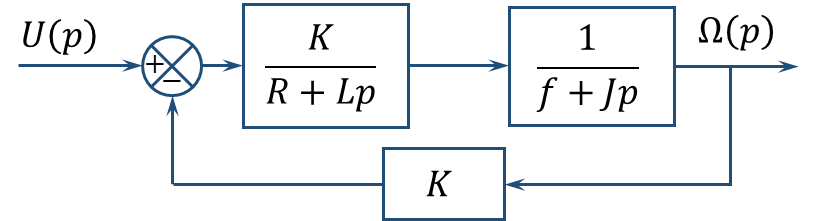
\includegraphics[width=.9\linewidth]{500_01}
\end{center}
 \fi
 
\question{Déterminer la fonction de transfert en boucle ouverte. Mettre l'expression sous forme canonique et exprimer les paramètres caractéristiques.}
\ifprof
On a $\text{FTBO}(p)=\dfrac{K^2}{\left(R+Lp\right)\left(f+Jp\right)}$
$=\dfrac{K^2}{Rf+RJp+Lfp+LJp^2}$
$=\dfrac{K^2}{Rf\left(1+p\dfrac{RJ+Lf}{Rf}+\dfrac{LJ}{Rf}p^2\right)}$.

On a donc $K_{\text{BO}}=\dfrac{K^2}{Rf}$, 
$\omega_{\text{BO}} = \sqrt{\dfrac{Rf}{LJ}}$,
$\dfrac{2\xi_{\text{BO}} }{\omega_{\text{BO}}}=\dfrac{RJ+Lf}{Rf} \Leftrightarrow
\xi_{\text{BO}} =\omega_{\text{BO}}\dfrac{RJ+Lf}{2Rf}
=\sqrt{\dfrac{Rf}{LJ}}\dfrac{RJ+Lf}{2Rf}
=\dfrac{RJ+Lf}{2\sqrt{LJRf}}$.
\else 
\fi

\question{Déterminer la fonction de transfert en boucle fermée. Mettre l'expression sous forme canonique et exprimer les paramètres caractéristiques.}
\ifprof
On a $\text{FTBF}(p)=\dfrac{\dfrac{K}{\left(R+Lp\right)\left(f+Jp\right)}}{1+\dfrac{K^2}{\left(R+Lp\right)\left(f+Jp\right)}}
=\dfrac{K}{\left(R+Lp\right)\left(f+Jp\right)+K^2}
=\dfrac{\dfrac{K}{K^2+Rf}}{\dfrac{RJ+Lf}{Rf+K^2}p+\dfrac{LJ}{Rf+K^2}p^2+1}$.



On a donc $K_{\text{BF}}=\dfrac{K}{K^2+Rf}$, 
$\omega_{\text{BF}} = \sqrt{\dfrac{Rf+K^2}{LJ}}$,
$\dfrac{2\xi_{\text{BF}} }{\omega_{\text{BF}}}=\dfrac{RJ+Lf}{Rf+K^2} \Leftrightarrow
\xi_{\text{BO}} =\omega_{\text{BF}}\dfrac{RJ+Lf}{2\left(Rf+K^2\right)}
=\sqrt{\dfrac{Rf+K^2}{LJ}}\dfrac{RJ+Lf}{2\left(Rf+K^2\right)}$
%=\sqrt{\dfrac{Rf}{LJ}}\dfrac{RJ+Lf}{2Rf}
%=\dfrac{RJ+Lf}{2\sqrt{LJRf}}$.
%
$\xi_{\text{BF}}=\dfrac{RJ+Lf}{2\sqrt{LJ}\sqrt{Rf+K^2}}$.
\else 
\fi

\ifprof 
\else
Soit le schéma-blocs suivant.
\begin{center}
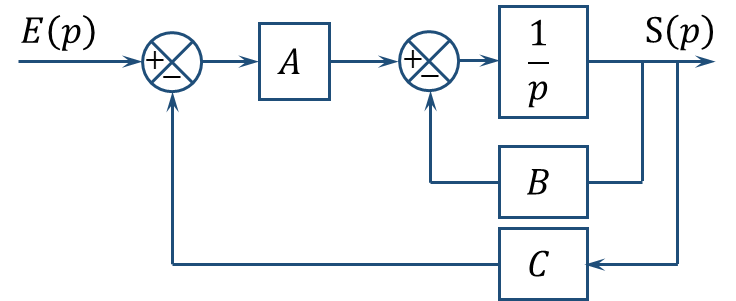
\includegraphics[width=.9\linewidth]{500_02}
\end{center}
 \fi
 
 \question{Déterminer la fonction de transfert en boucle ouverte. Mettre l'expression sous forme canonique et exprimer les paramétres caractéristiques.}
\ifprof
Si on note $R(p)$ la seconde entrée du \textbf{premier comparateur} et $\varepsilon(p)$ la sortie du premier comparateur,  

$\text{FTBO(p)}=\dfrac{\varepsilon(p)}{R(p)} = A \times \dfrac{\dfrac{1}{p}}{1+\dfrac{B}{p}}\times C = \dfrac{AC}{B+p} = \dfrac{\dfrac{AC}{B}}{1+\dfrac{p}{B}}$.
On a donc $K_{\text{BO}}=\dfrac{AC}{B}$ et $\tau_{\text{BO}}=\dfrac{1}{B}$.

\else 
\fi

 
\question{Déterminer la fonction de transfert en boucle fermée. Mettre l'expression sous forme canonique et exprimer les paramétres caractéristiques.}
\ifprof
On a
$\text{FTBF(p)} = \dfrac{\dfrac{A}{B+p}}{1+\dfrac{AC}{B+p}}=\dfrac{A}{B+p+AC}=\dfrac{\dfrac{A}{B+AC}}{1+\dfrac{p}{B+AC}}$.

On a donc $K_{\text{BF}}=\dfrac{A}{B+AC}$ et $\tau_{\text{BF}}=\dfrac{1}{B+AC}$.

\else 
\fi


%\question{Réaliser le schéma-blocs.}
%\ifprof
%\begin{figure}[H]
%\centering
%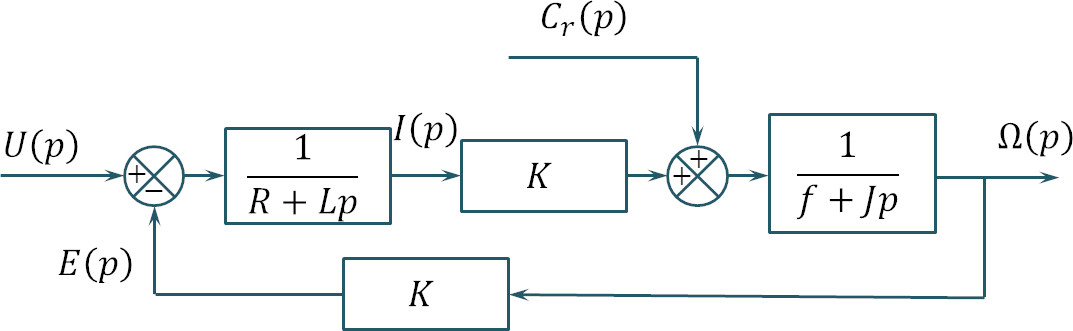
\includegraphics[width=\linewidth]{51_01_c}
%%\caption{Évolution du couple utile en fonction de la vitesse de rotation pour des
%%fréquences de commande de \SI{90}{Hz} à \SI{110}{Hz}. \label{fig_50_04}}
%\end{figure}
%\else
%\fi


 

\ifprof
\else
\footnotesize

\noindent
\begin{tabular}{|p{.9\linewidth}|}
\hline
Indications
\begin{enumerate}
\item $K_{\text{BO}}=\dfrac{K^2}{Rf}$, 
$\omega_{\text{BO}} = \sqrt{\dfrac{Rf}{LJ}}$,
$\xi_{\text{BO}} =\dfrac{RJ+Lf}{2\sqrt{LJRf}}$.
\item $K_{\text{BF}}=\dfrac{K}{K^2+Rf}$, 
$\xi_{\text{BF}}=\dfrac{RJ+Lf}{2\sqrt{LJ}\sqrt{Rf+K^2}}$.
\item $K_{\text{BO}}=\dfrac{AC}{B}$ et $\tau_{\text{BO}}=\dfrac{1}{B}$.
\item $K_{\text{BF}}=\dfrac{A}{B+AC}$ et $\tau_{\text{BF}}=\dfrac{1}{B+AC}$.
\end{enumerate} \\
\hline
\end{tabular}
\normalsize
\begin{flushright}
\footnotesize{Corrigé  voir \ref{B2:07:500}.}
\end{flushright}%
\fi